\section{Phantom}
The latest research \cite{phantom}\cite{bunnyhop} shows that modern x86 processors make predictions very early in the pipeline, even before the current instruction is decoded. Although this aggressive mechanism could improve CPU performance, it leads to new risks that almost all types of instruction could be trained to trigger prefetch \cite{bunnyhop} and even speculative execution\cite{phantom} within the transient window between prefetch and frontend resteer. This new source of speculation results in a broader attack surface and thus has significant research value.

 Our goal is to investigate whether this issue also exists on RISC-V processors, e.g. XiangShan, as well as the potential attack methods based on this issue. 
 
 % More specifically, our aim is to address the following four questions on XiangShan Nanhu core.
 % \begin{itemize}
 %     \item How to set up the branch history to trigger misprediction?
 %     \item Which combinations of branch instructions can be trained to trigger misprediction? How long is the transient window?
 %     \item By choosing proper victim instruction and setting up branch history, can we extend window to enable transient execution of the following instruction?
 %     \item How can this issue be exploited for attacks?
 % \end{itemize}

\subsection{Phantom on x86}
\subsubsection{Instruction decode pipeline}

Figure \ref{fig:decode} shows a common frontend design in x86 processor. Firstly, Branch Prediction Unit(BPU) predicts next instruction's PC and issue a instruction fetch request to Instruction Fetch Unit(IFU). IFU then fetches corresponding instructions from ICache and dispatchs them to Decoder for uop translation. Finally, these uops are sent to backend to be executed.  

\begin{figure}
    \centering
    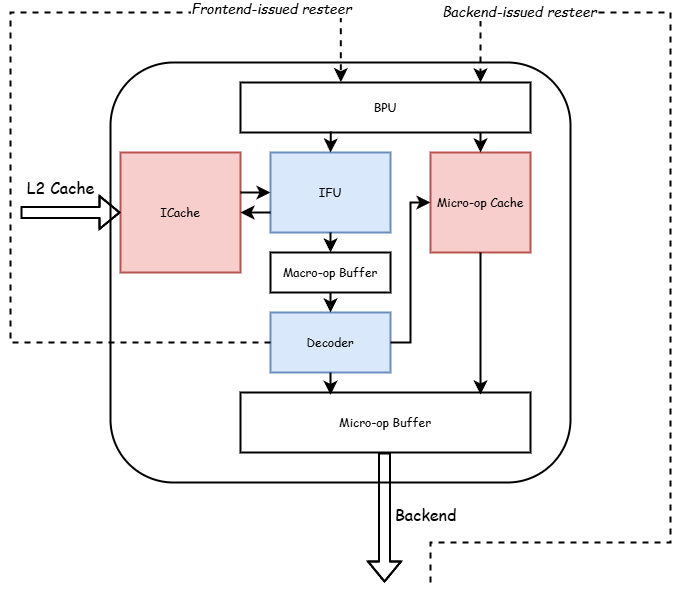
\includegraphics[width=0.4\textwidth]{Figure/decode pipeline.png}
    \caption{x86 Decode pipeline}
    \label{fig:decode}
\end{figure}

In the entire frontend pipeline, BPU plays a crucial role. For branch instructions that depend on the execution results from the backend to determine the jump address, the branch predictor predicts the jump address and sends a request to the IFU, prefetching the predicted instruction into the pipeline. Furthermore, to reduce the delay between instruction fetch and instruction decode, many branch predictors predict whether the current instruction is a branch instruction and also predict the address of the next instruction even before the current instruction is decoded.

In this design, there are two main sources of mispredictions: the mismatch of predicted instruction types, such as predicting a non-branch instruction as a branch instruction, or predicting a direct jump instruction as a branch/indirect jump instruction; and incorrect prediction of the branch instruction's behavior, such as whether a branch is taken or not, or the address of an indirect jump. The former can be detected during frontend instruction decoding, while the latter depends on the execution results of the relevant instructions in the backend.

When a misprediction is detected, a resteer signal is sent to the BPU, and the instruction pipeline is flushed (depending on the specific architecture design). The BPU then returns to the point where the misprediction occurred, corrects the mistake, and resumes pipeline.

While the execution-stage detectable misprediction often leaves a long enough transient execution window for subsequent instructions, which is exploited by the famous Spectre attack\cite{spectre}, recent research\cite{phantom} shows that the relatively short transient window caused by frontend misprediction could also make subsequent instructions enter the IF, ID, or even instruction execution.

\subsubsection{Observation Channels}
\label{sec:x86 phantom}

In order to better understand the frontend pipeline behavior of the instruction prefetch-decode stage and lay the ground for future work on RISC-V processors, we reproduced the experiments from the paper\cite{phantom} on AMD Zen2 and Zen3 processors. Due to the lack of open-source code from the original paper, we referred to several related works and leveraged our own understanding to develop the code. Additionally, there are some differences in the implementation design compared to the original paper.

The core of the experiment is to test the transient window length caused by mispredictions triggered by different instruction combinations set up for training/victim execution. This requires building up proper observation channels to track the advance of subsequent instructions through the pipeline. More specifically, we observe the progression of instructions through three stages in the pipeline: IF, ID, and EX.

\begin{figure}
    \centering
    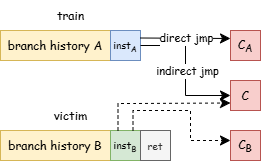
\includegraphics[width=0.3\textwidth]{Figure/trainning overview.png}
    \caption{Phantom Workflow}
    \label{fig:phantom workflow}
\end{figure}

The generic procedure is as follows. We have two snippets of code A and B, where A ends with a training branch to C. Branch A is either a direct jump/conditional jump instruction, where the target address is determined by a relative offset, or indirect jump instruction or return instruction, where the target address is specified by an absolute address in a register. For the former, we place code segment $\text{C}_\text{B}$ at the same offset as victim instruction B. We want to observe that running B after multiple executions of A causes a misprediction to $\text{C}_\text{B}$ / C that leads to detectable signals in IF, ID and EX observation channels.

\textbf{IF Channel}

We use Flush+Reload method \cite{flush_reload} to observe whether a instruction is brought into ICache. 

\begin{figure}[H]
    \centering
    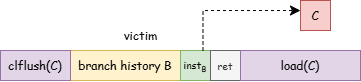
\includegraphics[width=0.4\textwidth]{Figure/IF Channel.png}
    \caption{IF Channel}
    \label{fig:IF Channel}
\end{figure}

Before testing B, we use the \texttt{clflush} instruction to flush the content at the misprediction address C from both the L1 and L2 caches. Next, we execute code snippet B to trigger the mis-branch to C. We then measure the time it takes to load C. A relatively short access time for C indicates that C's instruction has been prefetched into the L1-ICache, which serves as the IF channel.

\textbf{ID Channel}

Building ID Channel is a bit of tricky, since we cannot directly manipulate decoder and $\mu$op cache, since micro-op cache is independent of the memory subsystem. Alternatively, we use hardware performance counters to monitor instructions dispatched into $\mu$op cache.

\begin{figure}[H]
    \centering
    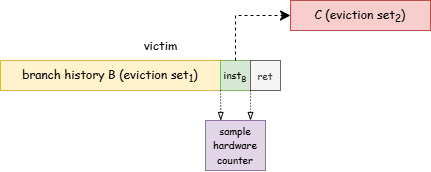
\includegraphics[width=0.4\textwidth]{Figure/ID Channel.png}
    \caption{ID Channel}
    \label{fig:ID Channel}
\end{figure}

As method provided in \cite{phantom}, we choose \textit{de\_dis\_uops\_from\_decoder.} \textit{de\_dis\_uops\_from\_opcache} on Zen2 and \textit{op\_cache\_hit\_miss.op\_cache\_miss} on Zen3. Follow the procedure illustrated in figure \ref{fig:ID Channel}, we first train A to jump to C which contains a series of direct jump instructions that will fill a certain $\mu$op cache set using method in \cite{dead_uop}. Then we execute B whose branch history also includes a direct jump series that maps to the same $\mu$op cache set as C maps to, which will replace the $\mu$op cache occupied by C. Finally, we sample the performance counter before and after B's execution. If a misprediction to C enter ID stage, it will result in eviction of one or more ways of the set, which is detectable using performance counters. By comparing the results with and without training, we can decide whether a misprediction occurred or not. In addition, on Zen2 we can directly use \textit{de\_dis\_uops\_from\_decoder.de\_dis\_uops\_from\_both} to monitor the differences in the number of uop instructions issued to backend to determine whether C's instructions are decoded.

In practice, the eviction jump series consists of 3~15  direct jumps separated by 2048 ~ 4096 bytes depending on the $\mu$op cache architecture.

\textbf{EX Channel}

\begin{figure}[H]
    \centering
    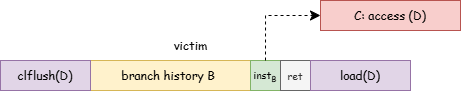
\includegraphics[width=0.4\textwidth]{Figure/EX Channel.png}
    \caption{EX Channel}
    \label{fig:EX Channel}
\end{figure}

To observe whether the transient window is long enough for instruction execution, we use a similar method in IF but by monitoring a memory access operation instead. That is, flush a cache line mapped to address D, execute B which might trigger a misprediction loading D from memory, and test the time to access D to determine whether a transient load occurred.  


\subsubsection{Triggering Misprediction}

To trigger a misprediction on B by training A, we must set them in the same branch history context, thus resulting in BTB (Branch Target Buffer) index aliasing. We follow the reverse engineering in previous work \cite{retbleed}, generating training address and victim address in pairs by flipping certain bits to create BTB collision. For AMD Zen2, we choose to flip the 19th bit and 31st bit, while for Zen3 21st bit and 33rd bit. Since AMD Zen2 and Zen3 use a relatively short branch history compared to Intel, 4~8 direct jumps are enough to craft a valid history.


\subsection{Phantom on RISC-V}
\subsubsection{Nanhu Frontend}
\begin{figure}[H]
    \centering
    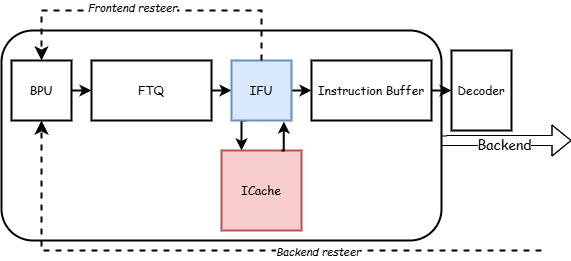
\includegraphics[width=0.4\textwidth]{Figure/xs-frontend.png}
    \caption{Nanhu Frontend}
    \label{fig:xs-frontend}
\end{figure}

As a RISC-V processor, the frontend of Xiangshan has two major differences compared to the typical x86 frontend:
\begin{itemize}
    \item Due to the fixed instruction length (4 bytes or 2 bytes for compressed instructions), the instruction decoding speed in RISC-V is relatively fast, so there is no need for a $\mu$op cache to accelerate decoding.
    \item Information such as whether the instruction is a branch instruction and the jump address can be obtained in the immediately after fetching the instruction through pre-decoding. Branch prediction checks are directly integrated into the IFU module.
\end{itemize}

As a result, once an instruction successfully enters the instruction buffer, it can be considered as being issued to the backend for execution.

Besdides, the open-source documentation of Xiangshan mentions that when a branch prediction error is detected, in addition to sending a redirection signal to the BPU, the entire IFU pipeline is flushed. This may result in a smaller transient window.

Therefore, our goal is to explore how this architectural change affects the transient window after a misprediction, as well as the instruction combinations that lead to mispredictions. Additionally, we aim to investigate whether this new architecture presents any potential issues.


\subsubsection{Observation Channels}

To determine how far an instruction advance in the pipeline, we select the IFU and Decoder as observation channels.

Although it is difficult to directly observe through methods like manipulating the cache or intervening the instruction pipeline, Xiangshan's rich set of frontend performance counters allows us to indirectly obtain a amount of information on instructions' status. Furthermore, since Xiangshan's code is fully open-source, we can directly modify the code to output the events we want to observe.

The training and testing process is similar to that of x86. Here, we will only introduce the observation metrics used.

\textbf{IFU}

For IFU, we mainly observe two events. Whether a instruction is brought into ICache and whether the IFU flush signal is triggered. The latter indicates that the misprediction is detected during the pre-decoding stage.

The corresponding registers are \textit{frontend\_icache\_miss\_cnt} and \textit{frontend\_flush}.

\textbf{Decoder}

We determine whether an instruction will be issued to the backend by monitoring the state of the decoder using \textit{ctrlblock\_decoder\_util-} \textit{-ization}, which records the total number of instructions decoded over a period of time.

The purpose of setting up this channel is to determine whether any instructions continue to be sent to the decoder during the period between the detection of a misprediction and the complete flush of the pipeline.

\textbf{EX}

We use same method to monitor instruction execution as mentioned in x86.

However, due to the significant noise in the hardware counters, simply using polling to sample may lead to discrepancies between the observed results and the actual situation\cite{hpc}. A more comprehensive test design is needed to ensure the reliability of the results.

\subsubsection{Triggering Misprediction}

As shown in figure \ref{fig:xs-branch-pred}, Xiangshan adopts a multi-level branch prediction design. Hence, to trigger a misprediction, we may need to mislead all levels of the predictor simultaneously.

Fortunately, perhaps to simplify the design, Xiangshan does not perform XOR hashing on the instruction's PC like Intel and AMD. Instead, it simply uses the lower bits of the PC XORed with the folded global history as the tag for the prediction table. To be more specific, $\mu$FTB uses PC's lower 16 bits as tag; TAGE-SC uses at most PC's lower 11 bits; FTB uses PC's lower 29 bits(9 for index and 20 for tag); ITTAGE uses at most lower 9 bits. Since XiangShan's overriding predictor design, the final prediction result is determined by ITTAGE, which means that matched 9 bits and 32 global history is enough to train a misprediction. Nevertheless, to avoid pipeline bubble caused by BPU redirection which might bring uncertainty to the experiment, We still choose to induce BTB aliasing by matching the lower 29 bits of PC.

\subsection{Exploitation Primitives}

We explore the possible exploitation primitives by examining the three stages of instruction advancement.

\subsubsection{IF}

Recent researches have proposed several techniques for exploiting the ICache, such as detecting executable memory \cite{phantom}, tracking cross-process / cross-privillege control flow \cite{bunnyhop} \cite{a-secure-risc}. These primitives are applicable on both x86 and RISC-V architectures.

\subsubsection{ID}

Although \cite{dead_uop} suggests that exploiting the $\mu$op cache can create sufficient instruction execution time differences to serve as a covert channel. To our knowledge, there is no known research that uses the $\mu$ op cache as a side channel for attacks. Since the $\mu$op cache is independent of the memory subsystem and hence less affected by noise interference, it might be possible to use the Prime + Probe method to more accurately track cross-process / cross-privilege instruction control flow. In addition, the $\mu$op cache may also serve as a channel for leaking other types of information. These possibilities require further research and experimentation. These primitives are only available on processor with $\mu$op cache, and thus may not be applied on the RISC-V CPU.

\subsubsection{EX}

The basic exploitation method is similar to that of typical speculative execution. However, Phantom execution means that more instruction combinations could be used to train speculative execution, and some defense mechanisms such as retpoline, which rely on software-level changes on indirect jump instructions, may become ineffective.



